\section{On-chip Network} \label{sec:network}

Achieving scalable performance using spatial architectures while supporting diverse applications requires a flexible, high-bandwidth interconnect.
  %Unfortunately, bandwidth and flexibility are often conflicting goals; static interconnects guarantee bandwidth but lack flexibility due to poor sharing.
  %Dynamic interconnects provide flexibility with better resource sharing but can cause bandwidth bottlenecks due to congestion while requiring more area and power.
 Because modern RDAs support vector units with wide datapaths, designing an interconnect that balances dynamism, communication granularity, and programmability is a challenging task.

On-chip interconnects can be classified into two broad categories: \emph{static} and \emph{dynamic.}
 {Static interconnects} use switches programmed at compile time to reserve high-bandwidth links between communicating units for the lifetime of the application.
RDAs traditionally employ static interconnects~\cite{cgraSurvey1, cgraSurvey2}.
In contrast, {dynamic interconnects}, or NoCs, contain routers that allow links to be shared between more than one pair of communicating units.
NoC communication is typically packet-switched, and routers use allocators to fairly share links between multiple competing packets.
Although static networks are fast, they require over-provision in bandwidth and can be underutilized
when a dedicated static link is reserved for a logical link that is not frequently active. 
While dynamic networks allow link sharing, the area and energy cost to transmit the same amount of data is higher for routers than for switches, making bandwidth scaling more expensive in dynamic networks than in static networks.

In this section, we explore the space of spatial architecture interconnect dynamism, granularity, and programmability.
We start by characterizing several benchmarks' communication patterns and showing links' imbalanced
bandwidth requirements, fanout, and data width in \Cref{sec:appchar}. 
Using these insights, we describe a hybrid network with both static and dynamic capabilities to enable both high bandwidth traffic and high resource sharing.
\Cref{sec:networkds} identifies a space of interconnection networks with static and dynamic capabilities, at multiple granularities. 
Next, We explain our methodology on performance, area, and power modeling in \Cref{sec:net_char}.
Finally, \Cref{sec:net_dse} perform a detailed evaluation of the identified design space for a variety of benchmarks.

Because RDAs encompass a broad range of architectures, we narrow our study on tile-based RDAs with
a streaming dataflow execution model, like Plasticine.
At high-level, the architecture may contain a pool of heterogeneous compute and memory tiles (we referring as 
physical units (PUs)) with a global network.
The network guarantees exactly-once, in-order delivery with variable latency, and communication 
between PUs can have varying granularities (e.g., 512-bit vector or 32-bit scalar).

To generalize the study, we introduce a variance in the style of processing engine (PE) in addition
to Plasticine's SIMD pipeline unit (pipelined RDA architecture).
The alternative style is a small vector processor that can execute a small loop of instructions repeatedly in
time (scheduled RDA architecture).
The scheduling window is small enough that instructions are stored as part of the configuration fabric, 
without dynamic instruction fetching overhead. 
Compared to the pipelined architecture, 
this execution model creates more interleaved pipelining across PUs with communication that is
tolerant of lower network throughput, which creates an opportunity for link sharing.

\subsection{Application Characteristics} \label{sec:appchar}
The requirements of an interconnection network are a function of the applications' communication
pattern, underlying RDA architecture, and compilation process.
We identify the following key characteristics of spatially mapped applications:

\paragraph{Vectorized communication}
Recent hardware accelerators use large-granularity compute tiles (e.g., vectorized compute units and SIMD pipelines) for
SIMD parallelism~\cite{plasticine, xilinx-acap}, which improves compute density while minimizing control and configuration overhead. 
Coarser-grained computation typically increases the size of communication, but glue logic, reductions, and loops with carried dependencies (i.e., non-parallelizable loops) contribute to scalar communications. 
This variation in communication motivates specialization for the optimal area- and energy-efficiency: separate networks for different communication granularities.

\paragraph{Broadcast and incast communication} 
A key optimization to achieve good performance on RDA is to explore multiple levels
of parallelization and pipelining, within and across PUs.
By default, pipeline parallelism across PUs introduces high-bandwidth one-to-one communication between dependent stages.
To balance the pipeline throughput, we often need to parallelize the pipeline stage with the most
computation, resulting in one-to-many communication when the receiver stage is parallelized, and
many-to-one communication when the producer stage is parallelized.
When both the producer and the consumer are parallelized, 
the worst case is many-to-many communication, as illustrated in \Cref{sec:memsplit}.
These broadcast and incast patterns introduce challenges in high-performance on-chip networks, as
their bandwidth demands scale quadratically with their chip size in the worst case.

\paragraph{Compute to memory communication}
To encourage better sharing of on-chip memory capacity, many accelerators have shared scratchpads, either distributed throughout the chip or on its periphery~\cite{plasticine, brainwave, streamdataflow}.
Because the compute unit has no local memory to buffer temporary results, the results of all computations are sent to memory through the network.
This differs from the NoCs used in multi-processors, where each core has a local cache to buffer intermediate results.
Studies have shown that for large-scale multiprocessor systems, network latency---not throughput---is the primary performance limiter~\cite{noc}.
For spatial accelerators, however, compute performance is limited by network throughput, and latency is comparatively less important.

\begin{figure}
\centering
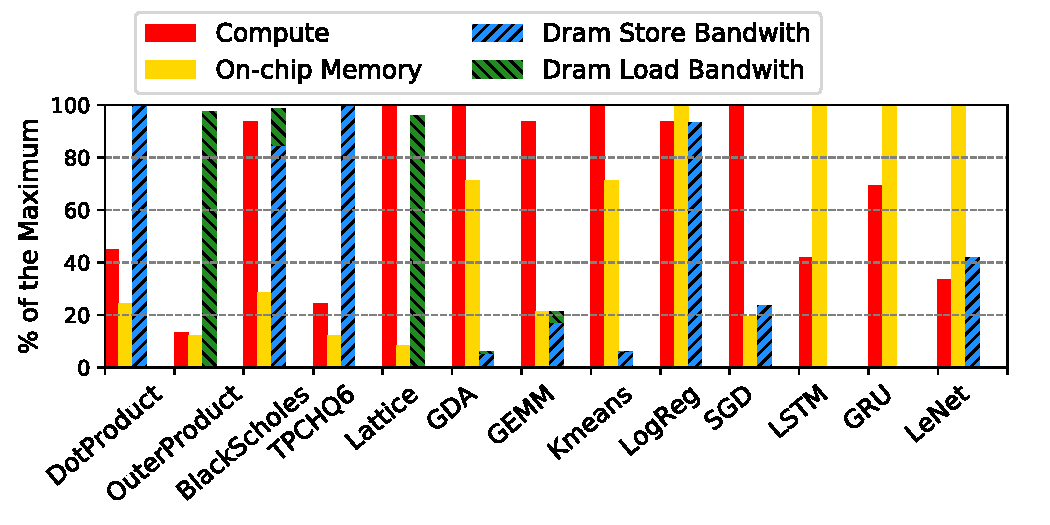
\includegraphics[width=0.8\columnwidth]{network/figs/util_bw2.pdf}
\caption[Resource and bandwidth utilization]{
  Physical resource and bandwidth utilization for various applications.}\label{fig:util_bw}
\centering
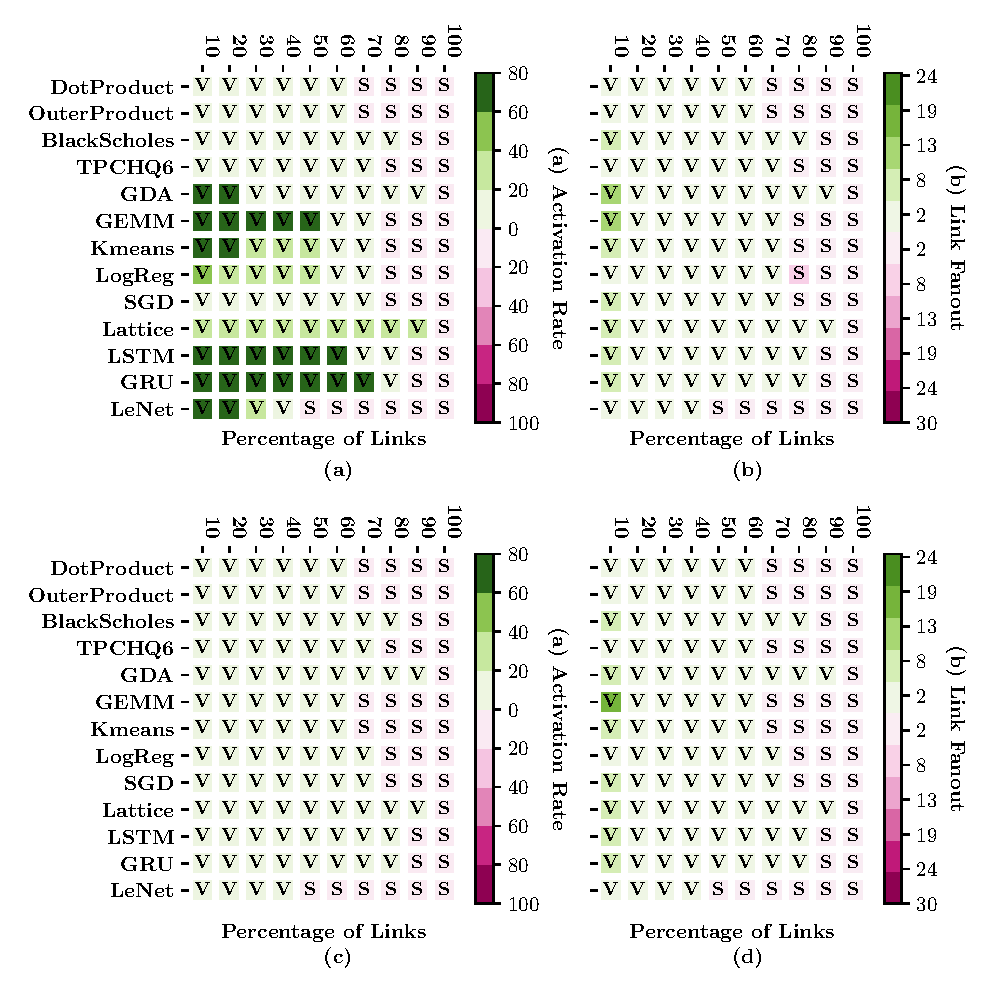
\includegraphics[width=0.8\columnwidth]{network/figs/link7.pdf}
  \caption[Application communication patterns]{Application communication patterns on pipelined (a,b) and scheduled (c,d) RDA architectures.
  (a) and (c) show the activation rate distribution of logical links at runtime. 
  Links sorted by granularity, then rate; darker boxes indicate higher rates.
  The split between green and pink shows the ratio of logical vector to scalar links. (b) and (d) show the distribution of broadcast link fanouts.
 }\label{fig:link}
\end{figure}

\begin{table*}
\centering
  \footnotesize
  \begin{tabular*}{6.25in}{p{0.75in} p{3in} p{2.5in}}
    \bottomrule
    \textbf{Benchmark} & \textbf{Description} & \textbf{Data Size} \\ \midrule
    DotProduct & Inner product & $1048576$ \\ \midrule
    OuterProduct & Outer product &$1024$ \\ \midrule
    BlackScholes & Option pricing &$1048576$ \\ \midrule
    TPCHQ6 & TPC-H query 6 &$1048576$ \\ \midrule
    Lattice & Lattice regression~\cite{garcia2009lattice} &$1048576$\\ \midrule
    GDA & Gaussian discriminant analysis &$127\times1024$ \\ \midrule
    GEMM & General matrix multiply &$256\times256\times256$ \\ \midrule
    Kmeans & K-means clustering &k=64, dim=64, n=8192, iter=2 \\ \midrule
    LogReg & Logistic regression &$8192\times128$, iter=4\\ \midrule
    SGD & Stochastic gradient descent for a single layer neural network &$16384\times64$, epoch=10 \\ \midrule
    LSTM & Long short term memory recurrent neural network &1 layer, 1024 hidden units, 10 time steps \\ \midrule
    GRU & Gated recurrent unit recurrent neural network &1 layer, 1024 hidden units, 10 time steps \\ \midrule
    LeNet & Convolutional neural network for character recognition& 1 image\\ \midrule
  \end{tabular*}
  \caption{Benchmark summary}
  \label{tab:benchmark}
\end{table*}

To study the communication patterns, 
we select a mix of applications from domains where hardware accelerators have shown promising performance and energy-efficiency benefits, such as linear algebra, databases, and machine learning.
Table~\ref{tab:benchmark} lists the applications and their data size.
Figure~\ref{fig:util_bw} shows, for each design, which resource limits performance: compute, on-chip memory, or DRAM bandwidth. 
DotProduct, TPCHQ6, OuterProduct, and BlackScholes are DRAM bandwidth-bound applications. 
These applications use few on-chip resources to achieve maximum performance, resulting in minimal communication.
Lattice (a fast inference model for low-dimensional regression~\cite{garcia2009lattice}), GDA, Kmeans, SGD, and LogReg are compute-intensive applications; for these, maximum performance requires using as much parallelization as possible. 
Finally, LSTM, GRU, and LeNet are applications that are limited by on-chip memory bandwidth or capacity. 
For compute- and memory-intensive applications, high utilization translates to a large interconnection network bandwidth requirement to sustain application throughput. 

Figure~\ref{fig:link}(a,b) shows the communication pattern of applications
characterized on the pipelined RDA architecture, including the variation in communication granularity. 
Compute and on-chip memory-bound applications show a significant amount of high-bandwidth communication (links with almost 100\% activity). 
A few of these high-bandwidth links also exhibit a high broadcast fanout. 
Therefore, a network architecture must provide sufficient bandwidth and efficient broadcasts to sustain program throughput.
On the contrary, time-scheduled architectures, shown in Figure~\ref{fig:link}(c,d), exhibit
lower bandwidth requirements due to the lower throughput of individual compute PUs. 
Even applications limited by on-chip resources have less than a 30\% firing rate on the busiest logical links; this reveals an opportunity for link sharing without sacrificing performance.

\begin{figure}
\centering
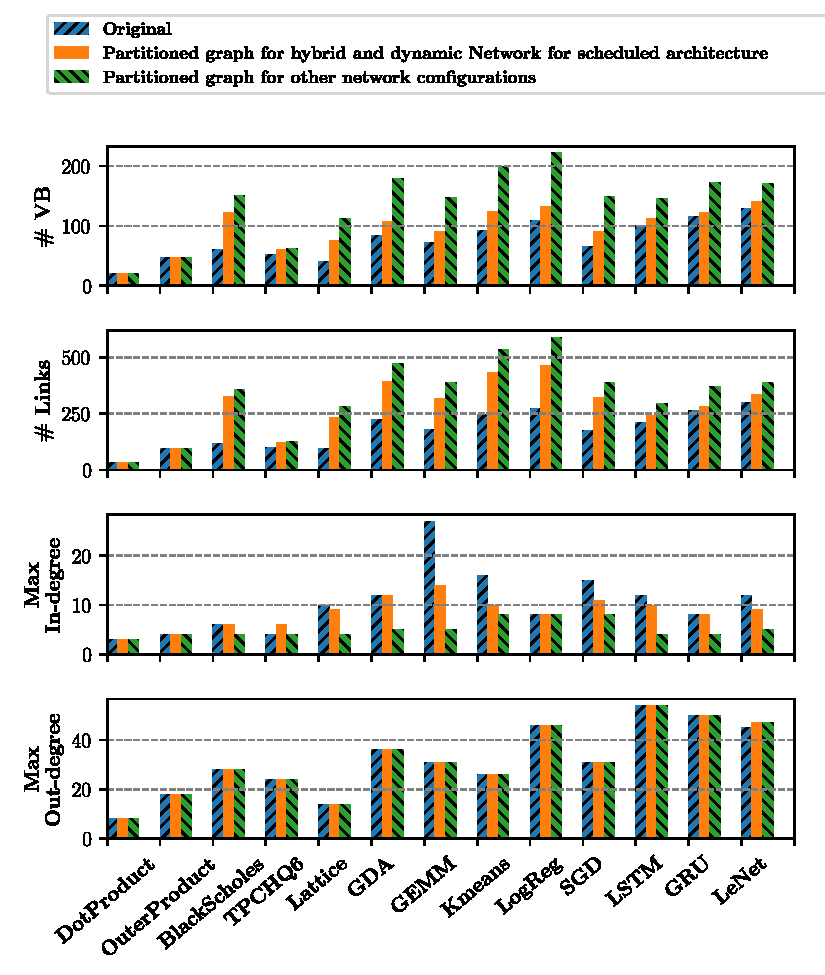
\includegraphics[width=0.9\columnwidth]{network/figs/graph.pdf}
\caption{Characteristics of program graphs.}\label{fig:graph}
\end{figure}

Figure~\ref{fig:graph} shows statistics describing the VU dataflow graph (VGDFG) before and after
the partitioning described in \Cref{sec:resalloc}. 
The blue bars show the number of VUs, number of logical links, and maximum VU input/output degrees in the original parallelized program; the yellow and green bars show the same statistics after partitioning. 
Fewer VUs are partitioned for hybrid networks and dynamic networks with the time-scheduled
architecture.
When a VU in a pipelined RDA consumes too many inputs or produces too many \emph{distinct} outputs,
\name partitions it to reduce its degree and meet the input/output bandwidth constraints of a purely static network. 
For dynamic and hybrid networks, partitioning is not strictly necessary, but it improves performance
by decreasing congestion at the network ejection port associated with a PU.
We do not partition broadcasts with high output degrees because they are handled natively within the network. 
Finally, the output degree does not change with partitioning because most outputs with a large degree are from broadcast links.

\subsection{Design Space for Network Architectures} \label{sec:networkds}

We start with several statically allocated network designs, where each SIMD pipeline connects to several switches, and vary flow control strategies and network bisection bandwidth.
In these designs, each switch output connects to exactly one switch input for the duration of the program.
We then explore a dynamic network, which sends program data as packets through an NoC.
The NoC uses a table-based routing scheme at each router to allow for arbitrary routes and tree-based broadcast routing.
Finally, we explore the benefits of specialization by evaluating design points that combine several of these networks to leverage the best features of each.

\subsubsection{Static networks}
We explore static network design points along three axes. 
First, we study the impact of flow-control schemes in static switches. 
In credit-based flow control~\cite{wang2013avoiding}, the source and destination PUs coordinate to ensure that the destination buffer does not overflow.
For this design point, switches only have a single register at each input, and there is no backpressure between switches.
The alternate design point uses a skid-buffered queue with two entries at each switch; using two entries enables per-hop backpressure and accounts for a one-cycle delay in stalling the upstream switch.
At full throughput, the receiver will consume data as it is sent and no queue will ever fill up.

The second axis studied is the bandwidth, and therefore routability, of the static network. 
We vary the number of connections between switches in each direction, which trades off area and energy for bandwidth.
Finally, we explore specializing static links: using a separate scalar network to improve routability at a low cost.

\subsubsection{Dynamic networks}
Our primary alternate design is a dynamic NoC using per-hop virtual channel flow control. 
Routing and Virtual Channel (VC) assignment are table-based: the compiler performs static routing and VC allocation, 
and results are loaded as a part of the routers' configurations at runtime.
The router has a separable, input-first VC and switch allocator with a single iteration and speculative switch allocation~\cite{dallytowles}.
Input buffers are sized just large enough (3 entries) to avoid credit stalls at full throughput.
Broadcasts are handled in the network with duplication occurring at the last router possible to minimize energy and congestion.
To respect the switch allocator's constraints, each router sends broadcasts to output ports sequentially and in a fixed order.
This is because the switch allocator can only grant one output port per input port in every cycle, and the RTL router's allocator does not have sufficient timing slack to add additional functionality.
We also explore different flit widths on the dynamic network, with a smaller bus taking multiple cycles to transmit a packet.

Because RDA networks are streaming---each PU pushes the result to the next PU(s) without explicit request---the network cannot handle routing schemes that may drop packets; otherwise, application data would be lost.
Because packet ordering corresponds directly to control flow, it is also imperative that all packets arrive in the order they were sent; this further eliminates adaptive or oblivious routing from consideration.
We limit our study of dynamic networks to statically placed and routed source routing due to these architectural constraints.
PUs propagate backpressure signals from their outputs to their inputs, so they must be considered as part of the network graph for deadlock purposes~\cite{hansson2007avoiding}.
Furthermore, each PU has fixed-size input buffers; these are far too small to perform high-throughput, end-to-end credit-based flow control in the dynamic network for the entire program \cite{wang2013avoiding}.
Practically, this means that no two logical paths may be allowed to conflict at \emph{any} point in the network; to meet this guarantee, VC allocation is performed to ensure that all logical paths traversing the same physical link are placed into separate buffers.

\subsubsection{Hybrid networks}
Finally, we explore hybrids between static and dynamic networks that run each network in parallel. 
During static place and route, the highest-bandwidth logical links from the program graph are mapped onto the static network; once the static network is full, further links are mapped to the dynamic network.
By using compiler knowledge to identify the relative importance of links---the link fanout and activation factor---hybrid networks can sustain the throughput requirement of most high-activation links while using the dynamic network for low-activation links.

\subsection{Performance, Area, and Energy Modeling} \label{sec:net_char}

Next section gives a quantitative analysis of the performance, area, and energy trade-offs involved 
in choosing a RDA network, using benchmarks showing in \Cref{tab:benchmark}.
This section outlines our methodology on how we capture the network performance, area, and energy in our evaluations.
\Cref{tab:notation} gives our notation for various network parameters discussed
in~\Cref{sec:networkds}.

\begin{table}
\footnotesize
  \centering
\begin{tabular*}{0.65\textwidth}{c l}
  \bottomrule
  \textbf{Notation} & \textbf{Description} \\\midrule
  $[$S,H,D$]$ & Static, hybrid, and dynamic network \\\midrule
  x<\#> & Static bandwidth on vector network (\#links between switches) \\\midrule
  %$s\#$ & Number of links between switches on static scalar network \\\midrule
  f<\#> & Flit width of a router or vector width of a switch \\\midrule
  v<\#> & Number of VC in router \\\midrule
  b<\#> & Number of buffers per VC in router \\\midrule
  $[$db,cd$]$ & Buffered vs. credit-based flow control in switch \\\midrule
  %$[Scheduled, Pipelined]$ & Time scheduled vs deep pipelined accelerator architectures \\\midrule
\end{tabular*}
\caption{Network design parameter summary.}
\label{tab:notation}
\end{table}

\subsubsection{Simulation}
We use a cycle-accurate simulator to model the pipeline and scheduling delay for the two types of architectures,
 integrated with DRAMSim \cite{dramsim} to model DRAM access latency. For static networks, we model
a distance-based delay for both credit-based and per-hop flow control. 
For dynamic networks, we integrate
our simulator with Booksim \cite{jiang2013detailed}, adding support for arbitrary source routing using look-up tables. 
Finally, to support efficient multi-casting in the dynamic network, we modify Booksim to duplicate broadcast packets at the router where their paths diverge.
At the divergence point, the router sends the same flit to multiple output ports over multiple cycles.
We assume each packet carries a unique ID that is used to look up the output port and next VC in a statically generated routing table, and that the ID is roughly the same size as an address.
When the packet size is greater than the flit size, the transmission of a single packet takes multiple cycles.

\subsubsection{Area and power}
To efficiently evaluate large networks, we start by characterizing the area and power consumption of individual routers and switches
used in various network configurations. 
The total area and energy are then aggregated over all switches and routers in a particular network.
We use router RTL from the Stanford open-source NoC router \cite{becker2012efficient} and our own parameterized switch implementation.
We synthesize using Synopsys Design Compiler with a \SI{28}{nm} technology library and clock-gating enabled, meeting timing at a 1 GHz clock frequency.
Finally, we use Synopsys PrimeTime to back-annotate RTL signal activity to the post-synthesis switch and router designs to estimate gate-level power.

We found that power consumption can be broken into two types: 
inactive power consumed when switches and routers are at zero-load ($P_{\text{inactive}}$, which includes both dynamic and static power),
and active power. The active power, as shown in Section~\ref{sec:net_char}, is proportional to the amount of
data transmitted. 
Because power scales linearly with the amount of data movement, we model the marginal energy to transmit a single flit of data (flit energy, $E_{\text{flit}}$) by dividing active energy by the number flits transmitted in the testbench:
\begin{equation}
  E_{\text{flit}} = \frac{\left(P-P_{\text{inactive}}\right) T_{\text{testbench}}}{\#\text{flit}} 
\end{equation}
While simulating an end-to-end application, we track the number of flits transmitted at each switch and router in the network, as well as the number of switches and routers allocated by place and route. 
We assume unallocated switches and routers are perfectly power-gated and do not consume energy.
The total network energy for an application on a given network ($E_{\text{net}}$) can be computed as:
\begin{equation}
  E_{\text{net}} = \sum_{\text{allocated}} P_{\text{inactive}} T_{\text{sim}}
  + E_{\text{flit}}  \#\text{flit},
\end{equation}
where $P_{\text{inactive}},$ $E_{\text{flit}},$ and $\#\text{flit}$ are tabulated separately for each network resource.

\begin{figure}
\centering
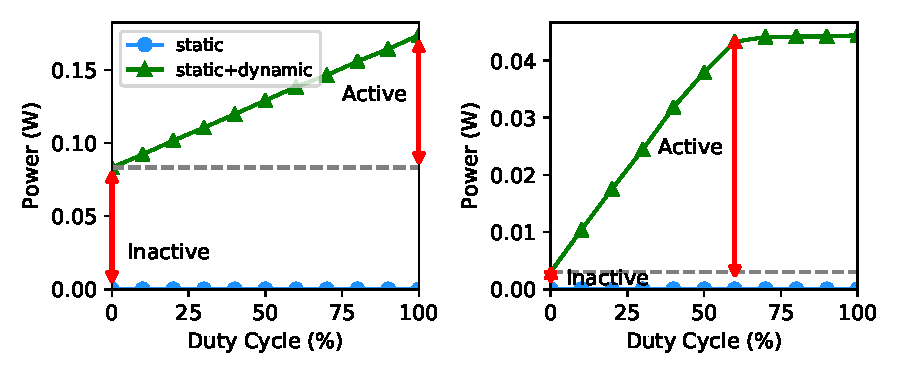
\includegraphics[width=0.8\columnwidth]{network/figs/sweep.pdf}
  \caption{Switch and router power with varying duty cycle.}\label{fig:sweep}
\end{figure}


Figure~\ref{fig:sweep} shows that switch and router power scale linearly with the rate of data transmission, but that there is non-zero power at zero-load. 
For simulation, the duty cycle refers to the amount of offered traffic, not accepted traffic.
Because our router uses a crossbar without speedup \cite{dallytowles}, the testbench saturates the router at 60\% duty cycle when providing uniform random traffic. 
Nonetheless, router power still scales linearly with accepted traffic.

A sweep of different switch and router parameters is shown in Figure~\ref{fig:char}. Subplots (d,e,f) show the energy necessary to transmit a single bit through a switch or router.
Subplot (a) shows the roughly quadratic scaling of switch area with the number of links between adjacent switches.
Vector switches scale worse with increasing bandwidth than scalar switches, mostly due to increased crossbar wire load. 
At the same granularity, a router consumes more energy a switch to transmit a single bit of data, even though the overall router consumes less power (as shown in Figure~\ref{fig:sweep}); 
this is because the switch has a higher throughput than the router.
The vector router has lower per-bit energy relative to the scalar router because it can amortize the cost of allocation logic, whereas the vector switch has higher per-bit energy relative to the scalar switch due to increased capacitance in the large crossbar. 
Increasing the number of VCs or buffer depth per VC also significantly increases router area and energy, but reducing the router flit width can significantly reduce the router area. 

\begin{figure}
\centering
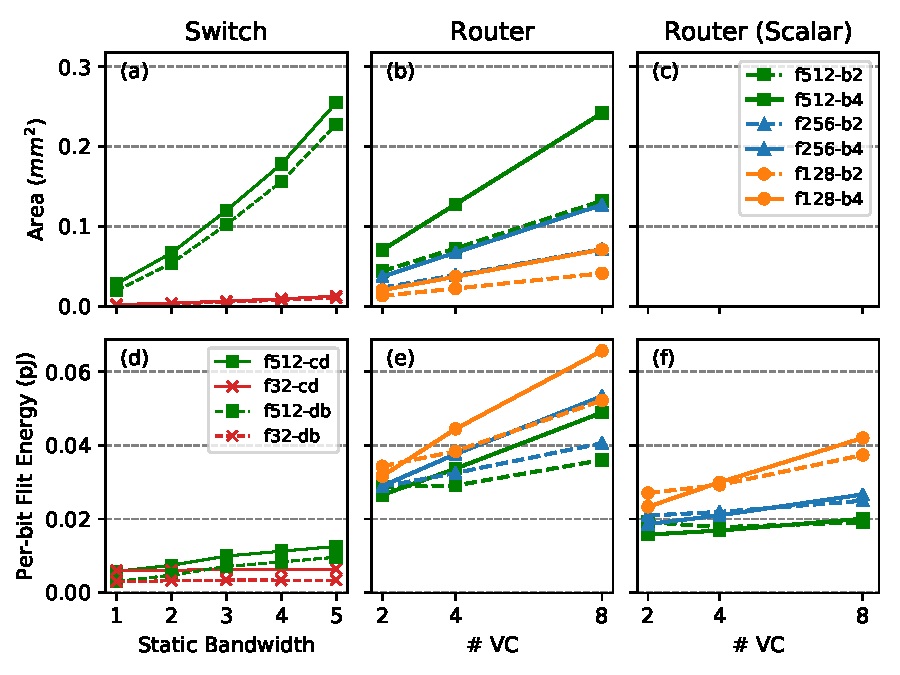
\includegraphics[width=0.8\columnwidth]{network/figs/char.pdf}
  \caption{Area and per-bit energy for (a,d) switches and (b,c,f) routers. 
  The router only has a vector granularity and can be partially clock-gated when sending scalar packets.
  Subplots (f) show the energy of the vector router when used for scalar values (32-bit).}\label{fig:char}
\end{figure}

Overall, these results show that scaling static bandwidth is cheaper than scaling dynamic bandwidth, and a dynamic network with small routers can be used to improve link sharing for low bandwidth communication.  
We also see that a specialized scalar network, built with switches, adds a negligible area compared to and is more energy-efficient than the vector network. 
Therefore, we use a static scalar network with a bandwidth of 4 for the remainder of our evaluation, except when evaluating the pure dynamic network.
The dynamic network is also optimized for the rare instances when the static scalar network is insufficient. 
When routers transmit scalar data, the high bits of data buffers are clock-gated, reducing energy as shown in (f).
Figure~\ref{fig:area} summarizes the area breakdown of all the network configurations that we evaluate.

\begin{figure}
\centering
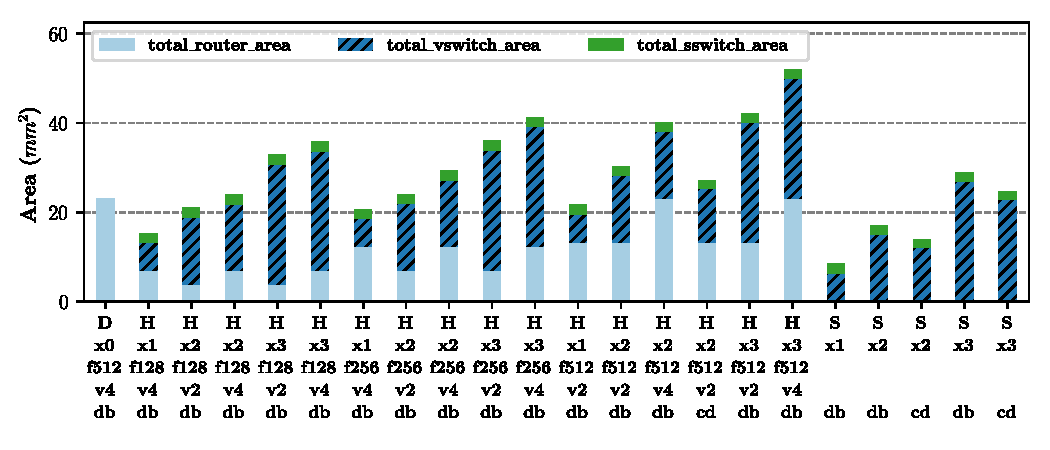
\includegraphics[width=1\columnwidth]{network/figs/area.pdf}
  \caption{Area breakdown for all network configurations.}\label{fig:area}
\end{figure}

\subsection{Network Architecture Evaluation} \label{sec:net_dse}

We evaluate our network configurations in five dimensions: performance (perf), performance per network area (perf/area), performance per network
power (perf/watt), network area efficiency (1/area), and network power efficiency (1/power). 
Among these metrics, performance is the most important: networks only consume a small fraction of the overall accelerator area and energy (roughly 10-20\%). 
Because the two key advantages of hardware accelerators are high throughput and low latency, 
we filter out a network design point if it introduces
more than 10\% performance overhead.
This is calculated by comparing to an ideal network with infinite bandwidth and zero latency.

For metrics that are calculated per application, such as performance, performance/watt, and power efficiency, we first normalize the metric with respect to the 
worst network configuration for that application. 
For each network configuration, we present a geometric mean normalized across all applications. 
For all of our experiments, except Section~\ref{sec:scale}, we use a network
size of $14\times14$ end-point PUs. All vector networks use a vectorization factor of 16 (\SI{512}{bit} messages).

\begin{figure}
\centering
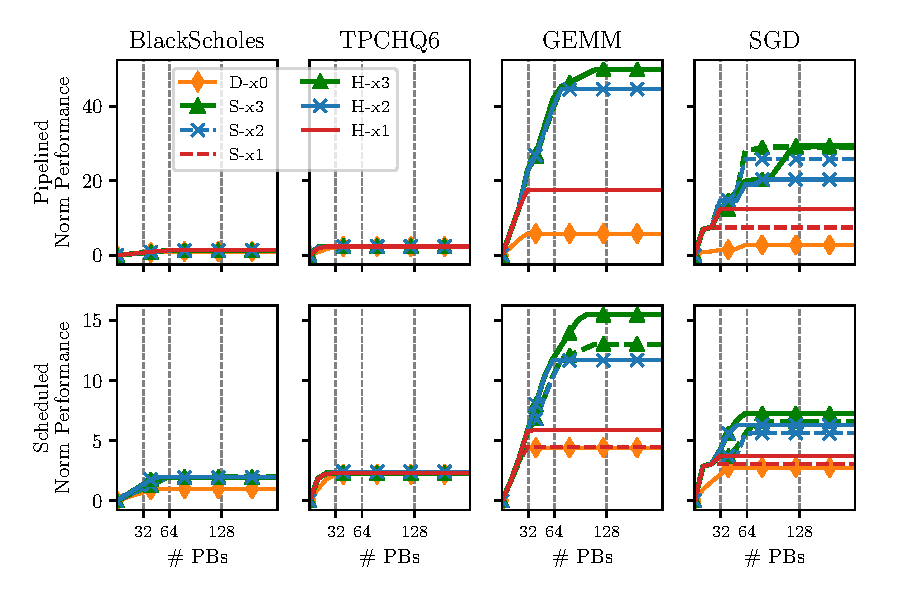
\includegraphics[width=0.8\columnwidth]{network/figs/scale.pdf}
\caption{Performance scaling with increased RDA grid size for different networks.}\label{fig:scale}
\end{figure}
\subsubsection{Bandwidth scaling with network size}\label{sec:scale}
Figure~\ref{fig:scale} shows how different networks allow several applications to scale to different numbers of PUs.
For IO-bound applications (BlackScholes and TPCHQ6), performance does not scale with additional compute and on-chip memory resources.
However, the performance of compute-bound applications (GEMM and SGD) improves with increased resources, but plateaus at a level that is determined by on-chip network bandwidth. 
This creates a trade-off in accelerator design between highly vectorized compute PUs with a small network---which would be underutilized for non-vectorized problems---and smaller compute PUs with limited performance due to network overhead. 
For more finely grained compute PUs, both more switches and more costly (higher-radix) switches must be employed to meet application requirements.

The scaling of time-scheduled accelerators (bottom row) is much less dramatic than that of deeply pipelined architectures (top row). 
Although communication between PUs in these architectures is less frequent, the scheduled architecture must use additional parallelization to match the throughput of the pipelined architecture; this translates to larger network sizes. 

For pipelined architectures, both hybrid and static networks provide similar scaling with the same static bandwidth:
the additional bandwidth from the dynamic network in hybrid networks does not provide additional scaling. 
This is mostly due to a bandwidth bottleneck between a PU and its router, which prevents the PU from requesting multiple elements per cycle.
Hybrid networks tend to provide better scaling for time-scheduled architectures; multiple streams can be time-multiplexed at each ejection port without losing performance.

\subsubsection{Bandwidth and flow control in switches}

\begin{figure}
  \centering
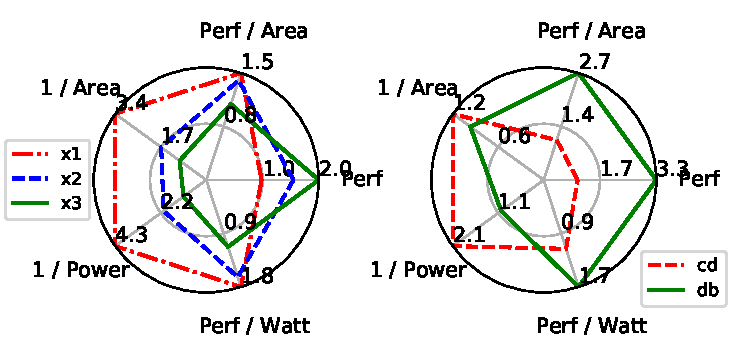
\includegraphics[width=0.7\textwidth]{network/figs/radar_switch.pdf}
  \caption{
    Impact of bandwidth and flow control strategies in switches.}\label{fig:radar_switch}
\end{figure}

In this section, we study the impact of static network bandwidth and flow control mechanisms (per-hop vs. end-to-end credit-based). 
On the left side of Figure~\ref{fig:radar_switch}, we show that increased static bandwidth results in a linear performance increase and a superlinear increase in area and power. 
As shown in Section~\ref{sec:scale}, any increase in accelerator size must be coupled with increased network bandwidth to effectively scale performance. 
This indicates that network overhead will increase with the size of an accelerator.

The right side of Figure~\ref{fig:radar_switch} shows that, although credit-based flow control reduces the amount of buffering in switches and decreases network area and energy, application performance is significantly impacted. 
This is the result of imbalanced data-flow pipelines in the program: when there are parallel long and short paths over the network, there must be sufficient buffer space on the short path equal to the product of throughput and the difference in latency. 
Because performance is our most important metric, credit-based flow control is not feasible, especially because the impact of bubbles increases with communication distance, and therefore network size.

\subsubsection{VC count and reduced flit width in routers}
\begin{figure}
  \centering
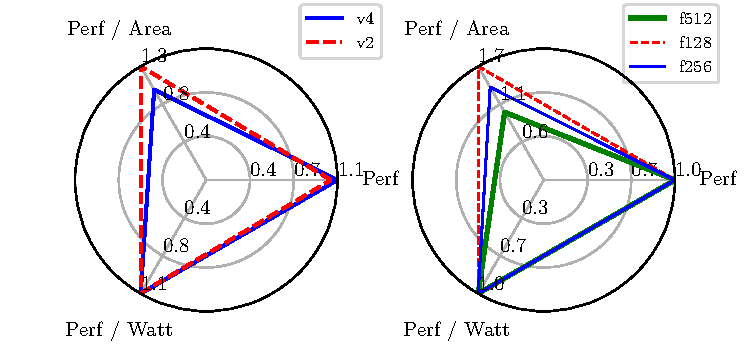
\includegraphics[width=0.7\textwidth]{network/figs/radar_router.pdf}
  \caption{Impact of VC count and flit widths in routers.}\label{fig:radar_router}
\end{figure}
In this experiment, we study the area-energy-performance trade-off between routers with different VC counts. As shown
in Section~\ref{sec:net_char}, using many VCs increases both network area and energy.
However, using too few VCs may force roundabout routing on the dynamic network or result in VC allocation failure when the network is heavily utilized.
Nonetheless, the left side of Figure~\ref{fig:radar_router} shows minimal performance improvement from using more VCs. 

Therefore, for each network design, we use a VC count equal to the maximum number of VCs required to map all applications to that network. 
Figure~\ref{fig:vc} shows that the best hybrid network configurations with 2x and 3x static bandwidth require at most 2 VCs, whereas the pure dynamic network requires 4 VCs to map all applications.
Because dynamic network communication is infrequent, hybrid networks with fewer VCs provide both better energy and area efficiency than networks with more VCs, even though this constrains routing on the dynamic network.

\begin{figure}
\centering
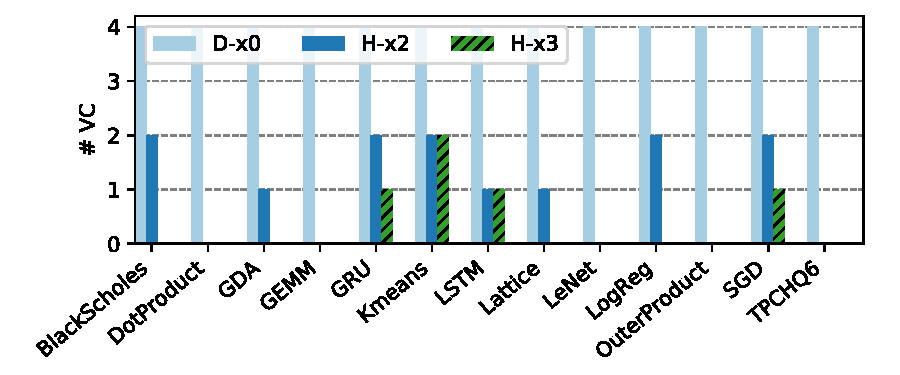
\includegraphics[width=0.75\textwidth]{network/figs/vc.pdf}
  \caption{Number of VCs required for dynamic and hybrid networks. (No VCs indicates that all traffic is mapped to the static network.)}\label{fig:vc}
\end{figure}

We also explore the effects of reducing dynamic network bandwidth by using smaller routers;
as shown in Section~\ref{sec:net_char}, routers with smaller flits have a much smaller area.
Ideally, we could scale static network bandwidth while using a low-bandwidth router to provide an escape path and reduce overall area and energy overhead. 
The right side of Figure~\ref{fig:radar_router} shows that, for a hybrid network, reducing flit width improves area efficiency with minimal performance loss. 

\subsubsection{Static vs. hybrid vs. dynamic networks}

\begin{figure*}
\centering
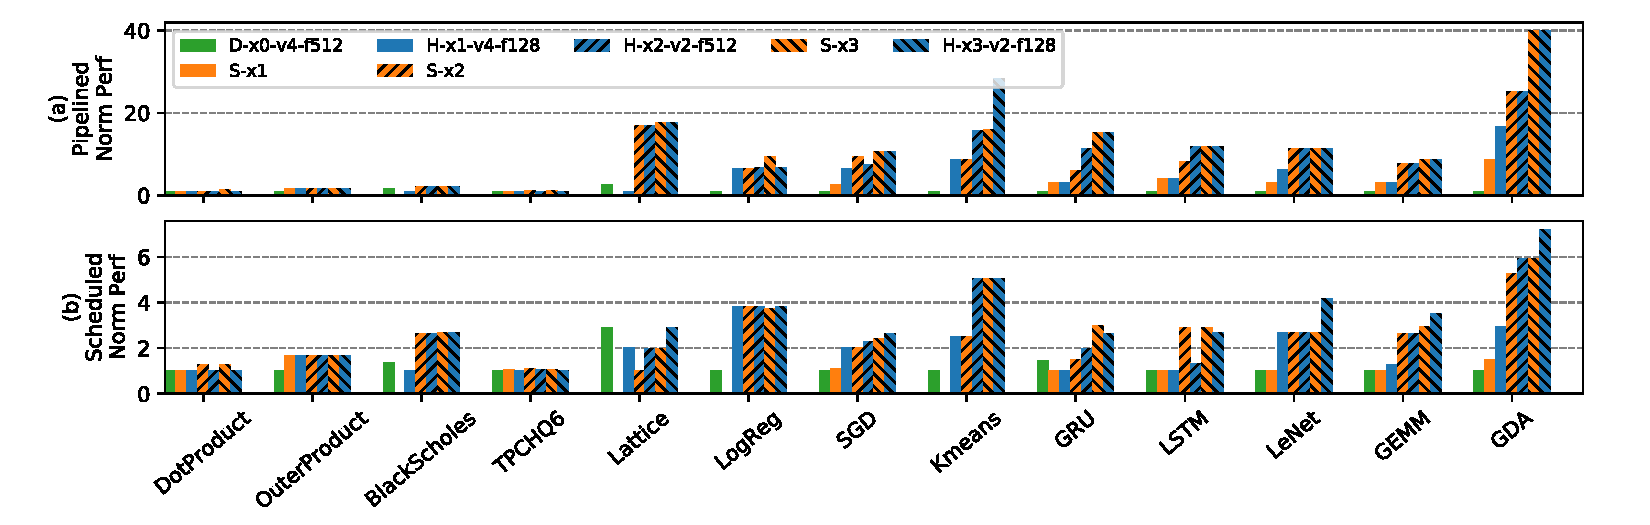
\includegraphics[width=1\linewidth]{network/figs/perf.pdf}
  \caption{Normalized performance for different network configurations.}\label{fig:perf}
\end{figure*}

Figure~\ref{fig:perf} shows the normalized performance for each application running on several network configurations.
For some applications, the bar for S-x1 is missing; this indicates that place and route failed for all unrolling factors.
For DRAM-bound applications, the performance variation between different networks is trivial because only a small fraction of the network is being used. 
In a few cases (Kmeans and GDA), hybrid networks provide better performance due to slightly increased bandwidth.
For compute-bound applications, performance primarily correlates with network bandwidth because more bandwidth permits a higher parallelization factor. 

\begin{figure}
\centering
  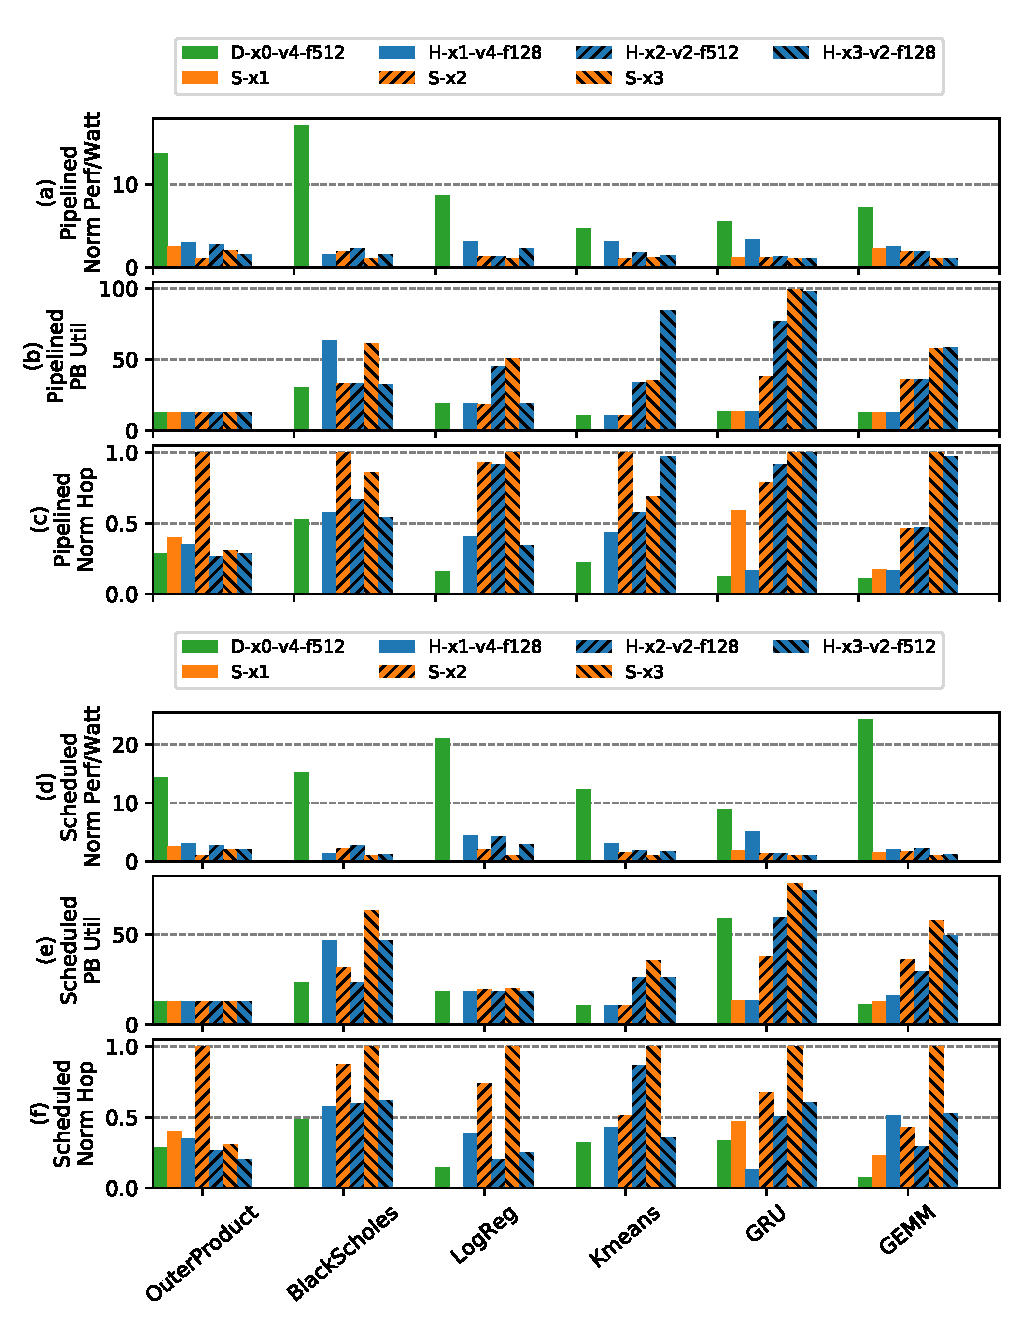
\includegraphics[width=0.9\textwidth]{network/figs/energy.pdf} 
\caption{(a,d): Normalized performance/watt. (b,e): Percentage of compute and memory PUs utilized for each network configuration. 
  (c,f): Total data movement (hop count).}
\label{fig:energy}
\end{figure}

The highest bandwidth static network uses the most PUs, as shown in Figures~\ref{fig:energy}(b,e), because it permits more parallelization. 
It also has more data movement, as shown in (c,f), because PUs can be distributed farther apart. 
Due to bandwidth limitations, low-bandwidth networks perform best with small unrolling factors---they are unable to support the bisection bandwidth of larger program graphs.
This is evident in Figures~\ref{fig:energy}(b,e), where networks D-x0-v4-f512 and S-x2 have small PU utilizations.

With the same static bandwidth, most hybrid networks have better energy efficiency than the corresponding pure static networks, even though routers take more energy than switches to transmit the same amount of data.
This is a result of allowing a small amount of traffic to escape onto the dynamic network: with the dynamic network as a safety net, static PaR tends to converge to better placements with less overall communication.
This can be seen in Figures~\ref{fig:energy}(c,f), where most static networks have larger hop counts than the corresponding hybrid network; hop count is the sum of all runtime link traversals, normalized per-application to the network configuration with the most hops.
Subplots (e,f) show that more PUs are utilized with static networks than hybrid networks.
This is because the compiler imposes less stringent IO constraints on PUs when partitioning for the hybrid network (as explained in Section~\ref{sec:partition}), which results in fewer PUs, less data movement, and greater energy efficiency for hybrid networks.

\begin{figure}
  \centering
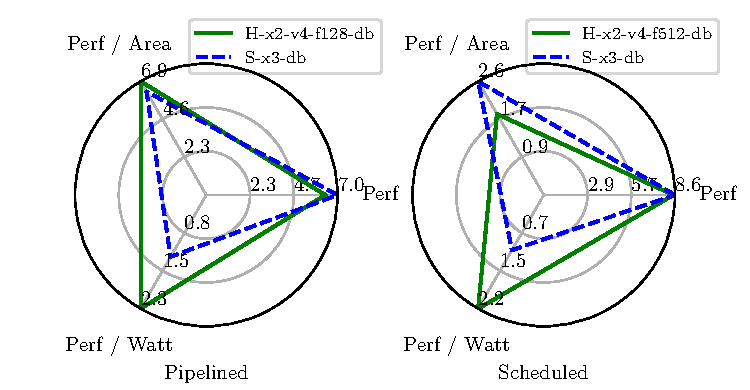
\includegraphics[width=0.7\textwidth]{network/figs/radar_best.pdf}
  \caption{Geometric mean improvement for the best network configurations, relative to the worst configuration.}\label{fig:radar_best}
\end{figure}
\begin{figure*}
\centering
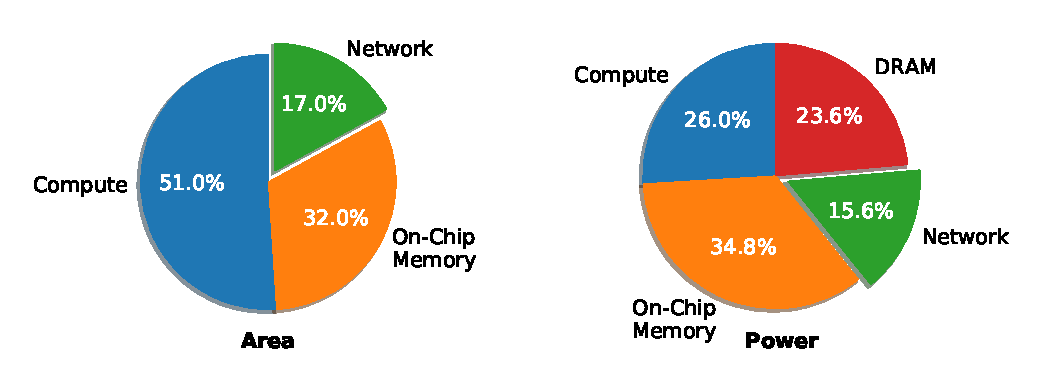
\includegraphics[width=0.8\textwidth]{figs/pie.pdf}
\caption[Area and power breakdown of Plasticine]{
  Area and power breakdown of Plasticine using a static-dynamic hybrid network.
}
\label{fig:breakdown}
\end{figure*}

In Figure~\ref{fig:radar_best}, we summarize the best perf/watt and perf/area (among network configurations with <10\% performance overhead) for pipelined and scheduled RDA architectures. 
Pure dynamic networks are not shown because they perform poorly due to insufficient bandwidth.
On the pipelined RDA, the best hybrid network provides a 6.4x performance increase, 2.3x better energy efficiency, and a 6.9x perf/area increase over the worst network configuration. 
The best static network provides 7x better performance, 1.2x better energy efficiency, and 6.3x better perf/area. 
The hybrid network gives the best perf/area and perf/watt, with a small degradation in performance when compared to the static network. 
On the time-scheduled RDA, both static and hybrid networks have an 8.6x performance improvement. 
The hybrid network gives a higher perf/watt improvement at 2.2x, whereas the static network gives a higher perf/area improvement at 2.6x.
Overall, the hybrid networks deliver better energy efficiency with shorter routing distances by allowing an escape path on the dynamic network.
